\section*{Tutorial 3}

\noindent
\begin{tikzpicture}
  \path ( 0,2) node [shape=circle,draw] {}
        ( 0,1) node [shape=circle,draw] {}
        ( 0,0) node [shape=circle,draw] {}
        ( 1,1) node [shape=rectangle,draw] {}
        (-1,1) node [shape=rectangle,draw] {};
\end{tikzpicture}

\noindent
\begin{tikzpicture}
  \node at ( 0,2) [circle,draw] {};
  \node at ( 0,1) [circle,draw] {};
  \node at ( 0,0) [circle,draw] {};
  \node at ( 1,1) [rectangle,draw] {};
  \node at (-1,1) [rectangle,draw] {};
\end{tikzpicture}

\noindent
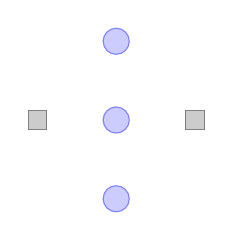
\begin{tikzpicture}
  \node at ( 0,2) [circle,draw=blue!50,fill=blue!20] {};
  \node at ( 0,1) [circle,draw=blue!50,fill=blue!20] {};
  \node at ( 0,0) [circle,draw=blue!50,fill=blue!20] {};
  \node at ( 1,1) [rectangle,draw=black!50,fill=black!20] {};
  \node at (-1,1) [rectangle,draw=black!50,fill=black!20] {};
\end{tikzpicture}

\noindent
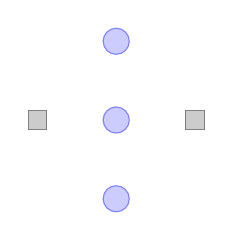
\begin{tikzpicture}
  [
    place/.style={circle,draw=blue!50,fill=blue!20},
    transition/.style={rectangle,draw=black!50,fill=black!20},
  ]
  \node at ( 0,2) [place] {};
  \node at ( 0,1) [place] {};
  \node at ( 0,0) [place] {};
  \node at ( 1,1) [transition] {};
  \node at (-1,1) [transition] {};
\end{tikzpicture}

\noindent
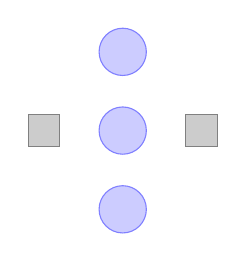
\begin{tikzpicture}
  [
    inner sep=0mm,
    place/.style={circle,draw=blue!50,fill=blue!20,minimum size=6mm},
    transition/.style={rectangle,draw=black!50,fill=black!20,minimum size=4mm},
  ]
  \node at ( 0,2) [place] {};
  \node at ( 0,1) [place] {};
  \node at ( 0,0) [place] {};
  \node at ( 1,1) [transition] {};
  \node at (-1,1) [transition] {};
\end{tikzpicture}

\noindent
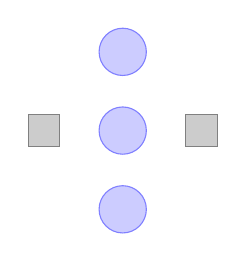
\begin{tikzpicture}
  [
    inner sep=0mm,
    place/.style={circle,draw=blue!50,fill=blue!20,minimum size=6mm},
    transition/.style={rectangle,draw=black!50,fill=black!20,minimum size=4mm},
  ]
  \node[place]      (waiting)        at ( 0,2)  {};
  \node[place]      (critical)       at ( 0,1)  {};
  \node[place]      (semaphore)      at ( 0,0)  {};
  \node[transition] (leave critical) at ( 1,1)  {};
  \node[transition] (enter critical) at (-1,1)  {};
\end{tikzpicture}

\noindent
\usetikzlibrary{positioning}
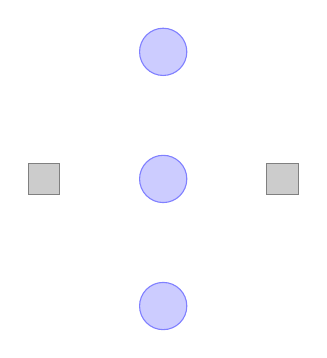
\begin{tikzpicture}
  [
    inner sep=0mm,
    place/.style={circle,draw=blue!50,fill=blue!20,minimum size=6mm},
    transition/.style={rectangle,draw=black!50,fill=black!20,minimum size=4mm},
  ]
  \node[place]      (waiting)                             {};
  \node[place]      (critical)       [below=of waiting]   {};
  \node[place]      (semaphore)      [below=of critical]  {};
  \node[transition] (leave critical) [right=of critical]  {};
  \node[transition] (enter critical) [left=of critical]   {};
\end{tikzpicture}

\noindent
\usetikzlibrary{positioning}
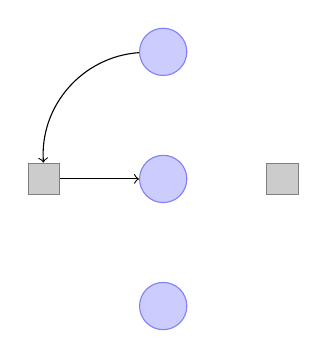
\begin{tikzpicture}
  [
    inner sep=0mm,
    place/.style={circle,draw=blue!50,fill=blue!20,minimum size=6mm},
    transition/.style={rectangle,draw=black!50,fill=black!20,minimum size=4mm},
  ]
  % Nodes placement
  \node[place]      (waiting)                             {};
  \node[place]      (critical)       [below=of waiting]   {};
  \node[place]      (semaphore)      [below=of critical]  {};
  \node[transition] (leave critical) [right=of critical]  {};
  \node[transition] (enter critical) [left=of critical]   {};
  % Connectors
 \draw[->] (enter critical) to                 (critical);
 %\draw[->] (waiting)        to [out=180,in=90] (enter critical);
 %\draw[->] (waiting)        to (enter critical);
 \draw[->] (waiting) to [bend right=45] (enter critical);
\end{tikzpicture}

\noindent
\usetikzlibrary{positioning}
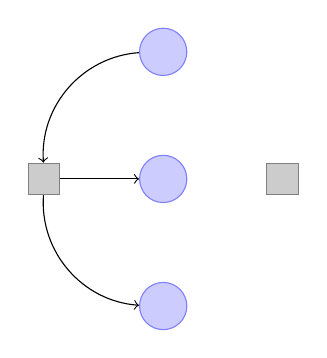
\begin{tikzpicture}
  [
    inner sep=0mm,
    place/.style={circle,draw=blue!50,fill=blue!20,minimum size=6mm},
    transition/.style={rectangle,draw=black!50,fill=black!20,minimum size=4mm},
  ]
  % Nodes placement
  \node[place]      (waiting)                             {};
  \node[place]      (critical)       [below=of waiting]   {};
  \node[place]      (semaphore)      [below=of critical]  {};
  \node[transition] (leave critical) [right=of critical]  {};
  \node[transition] (enter critical) [left=of critical]   {}
    edge[->]               (critical)
    edge[<-,bend left=45]  (waiting)
    edge[->,bend right=45] (semaphore);
\end{tikzpicture}

\noindent
\usetikzlibrary{positioning}
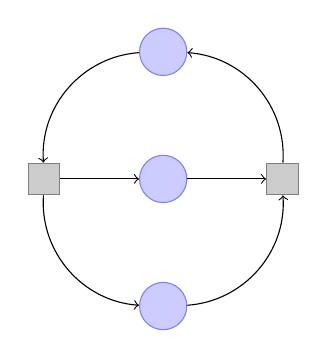
\begin{tikzpicture}
  [
    inner sep=0mm,
    place/.style={circle,draw=blue!50,fill=blue!20,minimum size=6mm},
    transition/.style={rectangle,draw=black!50,fill=black!20,minimum size=4mm},
    bend angle=45,
  ]
  
  % Nodes placement
  \node[place]      (waiting)                             {};
  \node[place]      (critical)       [below=of waiting]   {};
  \node[place]      (semaphore)      [below=of critical]  {};
  
  % Nodes with edges
  \node[transition] (leave critical) [right=of critical]  {}
    edge[<-]             (critical)
    edge[->, bend right] (waiting)
    edge[<-, bend left]  (semaphore);
  \node[transition] (enter critical) [left=of critical]   {}
    edge[->]             (critical)
    edge[<-,bend left]   (waiting)
    edge[->,bend right]  (semaphore);
\end{tikzpicture}